\documentclass{beamer}\usepackage[]{graphicx}\usepackage[]{color}
%% maxwidth is the original width if it is less than linewidth
%% otherwise use linewidth (to make sure the graphics do not exceed the margin)
\makeatletter
\def\maxwidth{ %
  \ifdim\Gin@nat@width>\linewidth
    \linewidth
  \else
    \Gin@nat@width
  \fi
}
\makeatother

\definecolor{fgcolor}{rgb}{0.345, 0.345, 0.345}
\newcommand{\hlnum}[1]{\textcolor[rgb]{0.686,0.059,0.569}{#1}}%
\newcommand{\hlstr}[1]{\textcolor[rgb]{0.192,0.494,0.8}{#1}}%
\newcommand{\hlcom}[1]{\textcolor[rgb]{0.678,0.584,0.686}{\textit{#1}}}%
\newcommand{\hlopt}[1]{\textcolor[rgb]{0,0,0}{#1}}%
\newcommand{\hlstd}[1]{\textcolor[rgb]{0.345,0.345,0.345}{#1}}%
\newcommand{\hlkwa}[1]{\textcolor[rgb]{0.161,0.373,0.58}{\textbf{#1}}}%
\newcommand{\hlkwb}[1]{\textcolor[rgb]{0.69,0.353,0.396}{#1}}%
\newcommand{\hlkwc}[1]{\textcolor[rgb]{0.333,0.667,0.333}{#1}}%
\newcommand{\hlkwd}[1]{\textcolor[rgb]{0.737,0.353,0.396}{\textbf{#1}}}%
\let\hlipl\hlkwb

\usepackage{framed}
\makeatletter
\newenvironment{kframe}{%
 \def\at@end@of@kframe{}%
 \ifinner\ifhmode%
  \def\at@end@of@kframe{\end{minipage}}%
  \begin{minipage}{\columnwidth}%
 \fi\fi%
 \def\FrameCommand##1{\hskip\@totalleftmargin \hskip-\fboxsep
 \colorbox{shadecolor}{##1}\hskip-\fboxsep
     % There is no \\@totalrightmargin, so:
     \hskip-\linewidth \hskip-\@totalleftmargin \hskip\columnwidth}%
 \MakeFramed {\advance\hsize-\width
   \@totalleftmargin\z@ \linewidth\hsize
   \@setminipage}}%
 {\par\unskip\endMakeFramed%
 \at@end@of@kframe}
\makeatother

\definecolor{shadecolor}{rgb}{.97, .97, .97}
\definecolor{messagecolor}{rgb}{0, 0, 0}
\definecolor{warningcolor}{rgb}{1, 0, 1}
\definecolor{errorcolor}{rgb}{1, 0, 0}
\newenvironment{knitrout}{}{} % an empty environment to be redefined in TeX

\usepackage{alltt}


\definecolor{deepcarmine}{rgb}{0.66, 0.13, 0.24}
\usepackage{pdfpc-movie}
\usetheme{Madrid}
\usecolortheme[named=deepcarmine]{structure}
\usefonttheme[onlymath]{serif}
\usepackage{tikz, amsfonts}
\usepackage{xcolor}
\usetikzlibrary{shapes.geometric, arrows}
\usepackage[natbib=true,
            style=nature,
            backend=biber,
            useprefix=true]{biblatex}
\usepackage{biblatex}
\addbibresource{references.bib}

\title[Modelling Cholera Treatments]
{Examining Treatment Strategies for Cholera Incorporating Spatial Dynamics}
\author[Plague Doctors]{Group: Plague Doctors \\ Jessa Mallare, Sid Reed, Daniel Segura, Aref Jadda}
\institute[McMaster]{McMaster University \and
Instructor: Dr. David Earn}
\date[April 8, 2019]{April 8, 2019}

\tikzstyle{blocks} = [rectangle, draw, rounded corners, text width=3em, text centered, minimum height=3em, fill = green!30]
\tikzstyle{blocki} = [rectangle, draw, rounded corners, text width=3em, text centered, minimum height=3em, fill = red!30]
\tikzstyle{blockr} = [rectangle, draw, rounded corners, text width=3em, text centered, minimum height=3em, fill = yellow!30]
\tikzstyle{blockb} = [rectangle, draw, rounded corners, text width=3em, text centered, minimum height=3em, fill = blue!30]
\tikzstyle{blank} = [inner sep=0,outer sep=0]
\tikzstyle{line} = [draw,->,>=stealth]
\IfFileExists{upquote.sty}{\usepackage{upquote}}{}
\begin{document}

\begin{frame}
\titlepage
\end{frame}

\begin{frame}{Introduction}
\begin{itemize}
\setlength\itemsep{2em}
\item Treatments have not always gone as planned in history
\item Cholera
\end{itemize}
\end{frame}

\begin{frame}{Some Biology on Cholera}
\begin{columns}[onlytextwidth]
\column{0.5\textwidth}
\begin{itemize}
\setlength\itemsep{2em}
\item \textit{Vibrio cholerae}
\item Colonizes the small intestine
\item 10 percent of infected individuals develop symptoms
\item Causes severe dehydration
\end{itemize}
\column{0.5\textwidth}
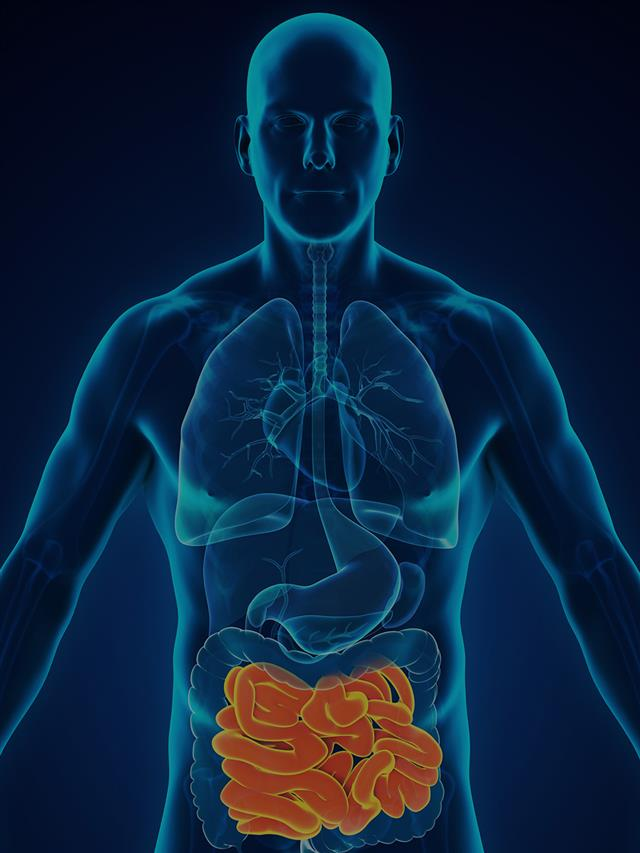
\includegraphics[width=0.65\textwidth]{images/SI.jpg}
\end{columns}
\end{frame}

\begin{frame}{Outbreaks in London ($19^{th}$ Century)}
\begin{columns}[onlytextwidth]
\column{0.5\textwidth}
\begin{itemize}
\setlength\itemsep{2em}
\item 1832, 1849, 1854, 1866
\item Miasma Theory
\item John Snow
\end{itemize}
\column{0.5\textwidth}
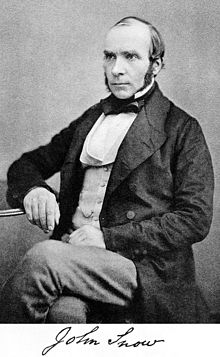
\includegraphics[width=0.65\textwidth]{images/Snow.jpg}
\end{columns}
\end{frame}

\begin{frame}{Developing a Single-Patch Model}
\begin{itemize}
\setlength\itemsep{2em}
\item Entire population (N) included
\item 3 Compartments : S, I, R
\item Compartment values are proportional
\item Water compartment for Cholera
\end{itemize}
\end{frame}

\begin{frame}{SIRW Model Assumptions}
\begin{itemize}
\setlength\itemsep{2em}
\item Birth Rate = Natural Death Rate and is constant
\item Population equally succeptible to infection
\item No waning immunity
\item No latency period
\item Only infected individuals can infect the water sources
\item Water sources can infect individuals
\end{itemize}
\end{frame}

\begin{frame}{SIRW Model}
\begin{center}
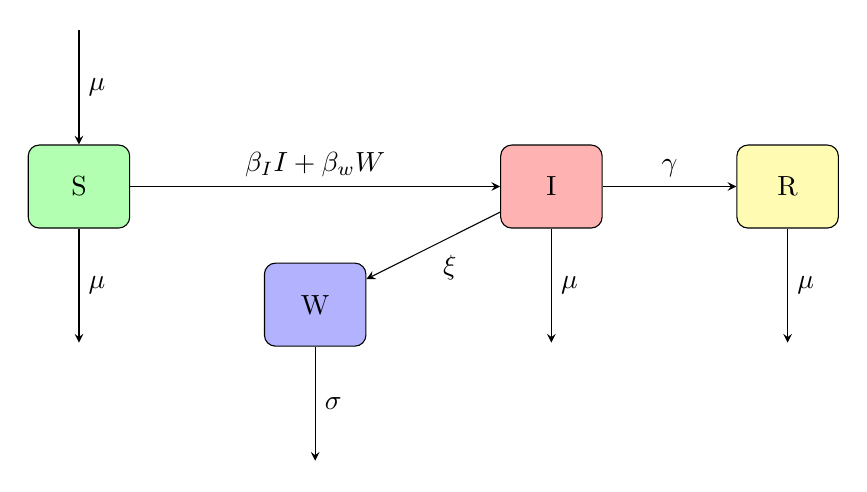
\begin{tikzpicture}[node distance=3cm, auto]

\node [blocks] (S) {S};
\node [blank, above of=S, yshift=-1cm] (0) { };
\node [blank, right of=S] (1) { };
\node [blockb, below of=1, yshift=1.5cm] (W) {W};
\node [blank, below of=W, yshift=1cm] (2) { };
\node [blocki, right of=1] (I) {I};
\node [blockr, right of=I] (R) {R};

\node [blank, below of=S, yshift=1cm] (3) {};
\node [blank, below of=I, yshift=1cm] (4) {};
\node [blank, below of=R, yshift=1cm] (5) {};

\path [line] (S) -- node {$\beta_I I + \beta_w W$} (I);
\path [line] (I) -- node {$\gamma$} (R);
\path [line] (I) -- node {$\xi$} (W);
\path [line] (W) -- node[anchor=west] {$\sigma$} (2);
\path [line] (0) -- node[anchor=west] {$\mu$} (S);

\path [line] (S) -- node[anchor=west] {$\mu$} (3);
\path [line] (I) -- node[anchor=west] {$\mu$} (4);
\path [line] (R) -- node[anchor=west] {$\mu$} (5);

\end{tikzpicture}
\end{center}
\end{frame}

\begin{frame}[t]{$R_0$ Calculation}
\begin{itemize}
\item Using the method of Next Generation Matrix (van den Driessche and Watmough, 2002)
\end{itemize}
\begin{align*}
		F&=\begin{pmatrix}
			\beta_i & \beta_w\\
			0 & 0
			\end{pmatrix}\\
		V&=\begin{pmatrix}
			\frac{1}{\gamma+\mu} & 0\\
			\frac{1}{\gamma+\mu} &\frac{1}{\sigma}
			\end{pmatrix}
\end{align*}
\begin{itemize}
\item $R_0$ is computed as the spectral radius of $FV^{-1}$:
\end{itemize}
\begin{align*}
    {\mathcal R_0} &= \rho(FV^{-1})\\
		           &=\frac{\beta_i+\beta_w}{\gamma+\mu} \approx 1.1 - 2.7
\end{align*}
\end{frame}

\begin{frame}{Equilibria and Stability}
\begin{itemize}
\setlength\itemsep{2em}
\item Two equilibria:\\[1em]
\begin{enumerate}
\setlength\itemsep{2em}
\item DFE: $(S,I,R)=(1,0,0)$
\item EE: $(S^{*},I^{*},R^{*}) = (\frac{1}{R_0}, \frac{\mu}{\gamma+\mu}(1-S^{*}), I^{*})$
\end{enumerate}
\item The DFE is stable when ${\mathcal R_0}<1$.
\item The EE is globally stable when ${\mathcal R_0}>1$ (Tien and Earn, 2010).
\end{itemize}
\end{frame}

\begin{frame}{SIWR Model Phase Portrait}
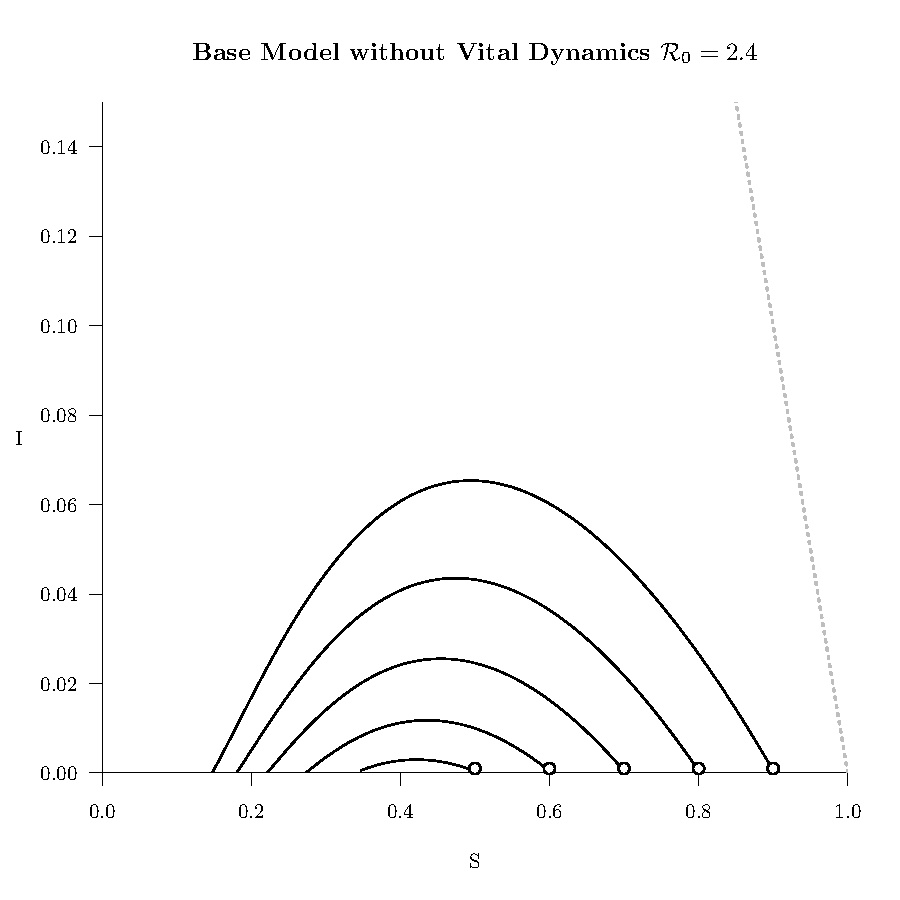
\includegraphics[width=0.475\textwidth]{images/phasebasewithoutvital.pdf}
\hfill
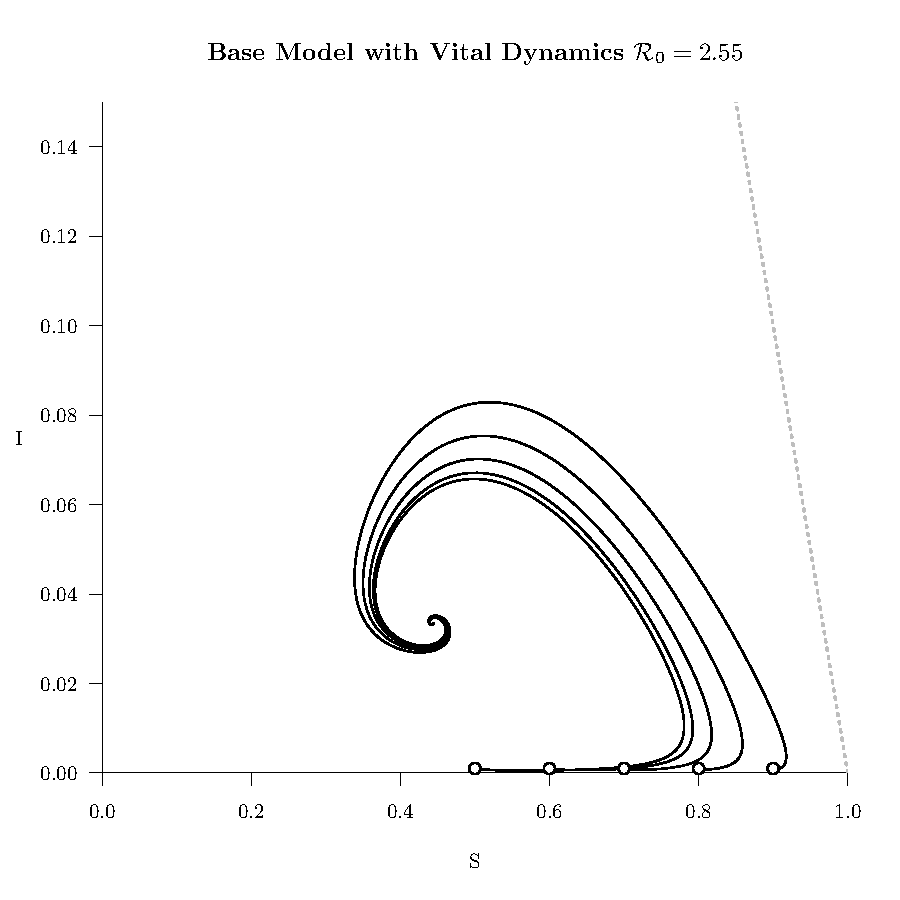
\includegraphics[width=0.475\textwidth]{images/phasebasewithvital.pdf}
%same parameter values between, only difference is \mu
%phasebase with vital R_0 = 2.255, phasebase without vital R_0=2.4
%vital dynamics shows damped oscillations to the EE
\end{frame}

\begin{frame}{Final Size}
\begin{columns}[onlytextwidth]
\column{0.5\textwidth}
\begin{itemize}
\setlength\itemsep{2em}
\item Assuming $\mu =0$ and $\mathcal R_0 > 1$, final size formula* still holds:
\item $Z = 1 - \exp{(-\mathcal R_0 Z - \frac{\beta_w}{\sigma}{w_0})}$
\end{itemize}
\column{0.5\textwidth}
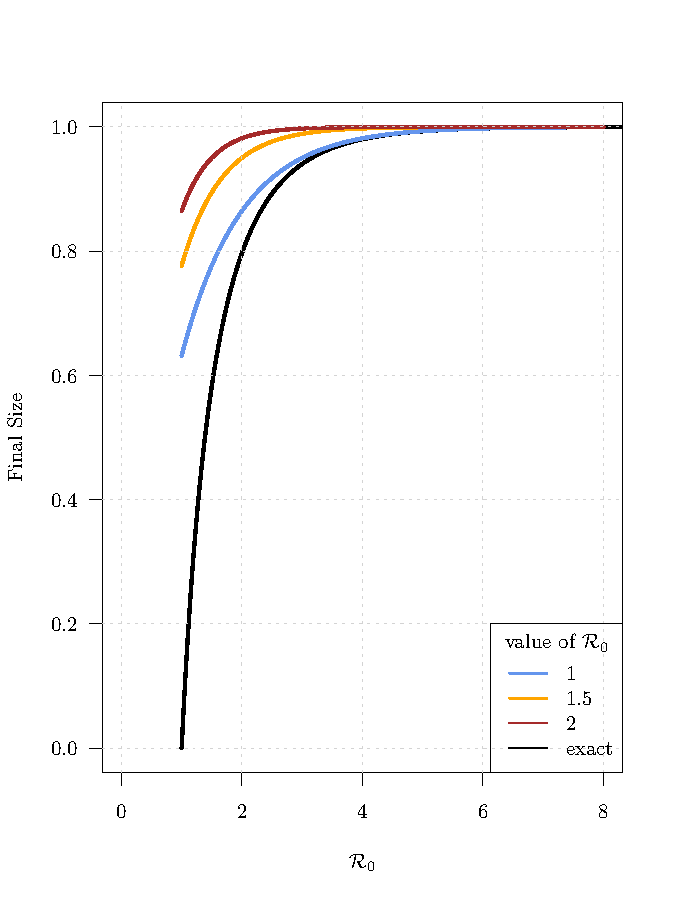
\includegraphics[width=0.95\textwidth]{images/finalsize.pdf}
\end{columns}
\end{frame}

\begin{frame}[t]{Effects of the 19th Century Treatments}
\begin{itemize}
\item Added parameter for death rate from Cholera: ($\alpha$)
\end{itemize}

\begin{center}
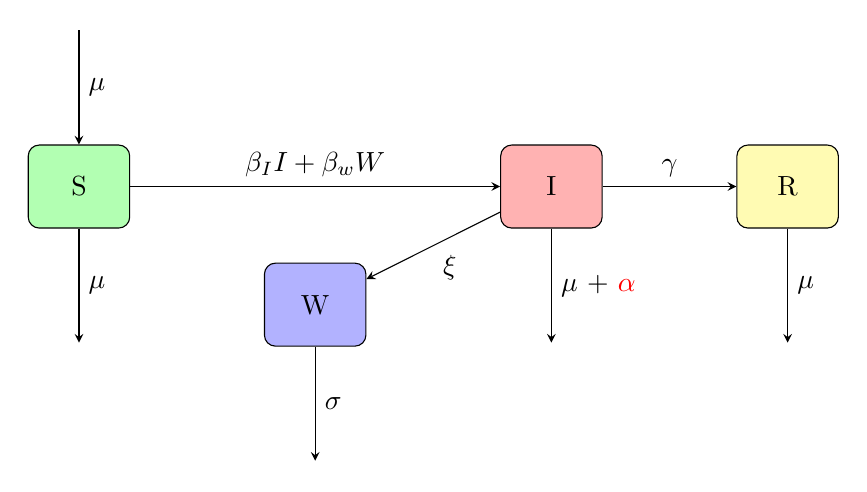
\begin{tikzpicture}[node distance=3cm, auto]

\node [blocks] (S) {S};
\node [blank, above of=S, yshift=-1cm] (0) { };
\node [blank, right of=S] (1) { };
\node [blockb, below of=1, yshift=1.5cm] (W) {W};
\node [blank, below of=W, yshift=1cm] (2) { };
\node [blocki, right of=1] (I) {I};
\node [blockr, right of=I] (R) {R};

\node [blank, below of=S, yshift=1cm] (3) {};
\node [blank, below of=I, yshift=1cm] (4) {};
\node [blank, below of=R, yshift=1cm] (5) {};

\path [line] (S) -- node {$\beta_I I + \beta_w W$} (I);
\path [line] (I) -- node {$\gamma$} (R);
\path [line] (I) -- node {$\xi$} (W);
\path [line] (W) -- node[anchor=west] {$\sigma$} (2);
\path [line] (0) -- node[anchor=west] {$\mu$} (S);

\path [line] (S) -- node[anchor=west] {$\mu$} (3);
\path [line] (I) -- node[anchor=west] {$\mu$ + \textcolor{red}{$\alpha$}} (4);
\path [line] (R) -- node[anchor=west] {$\mu$} (5);

\end{tikzpicture}
\end{center}
\end{frame}

\begin{frame}{Effects of the 19th Century Treatments}
\begin{columns}[onlytextwidth]
\column{0.5\textwidth}
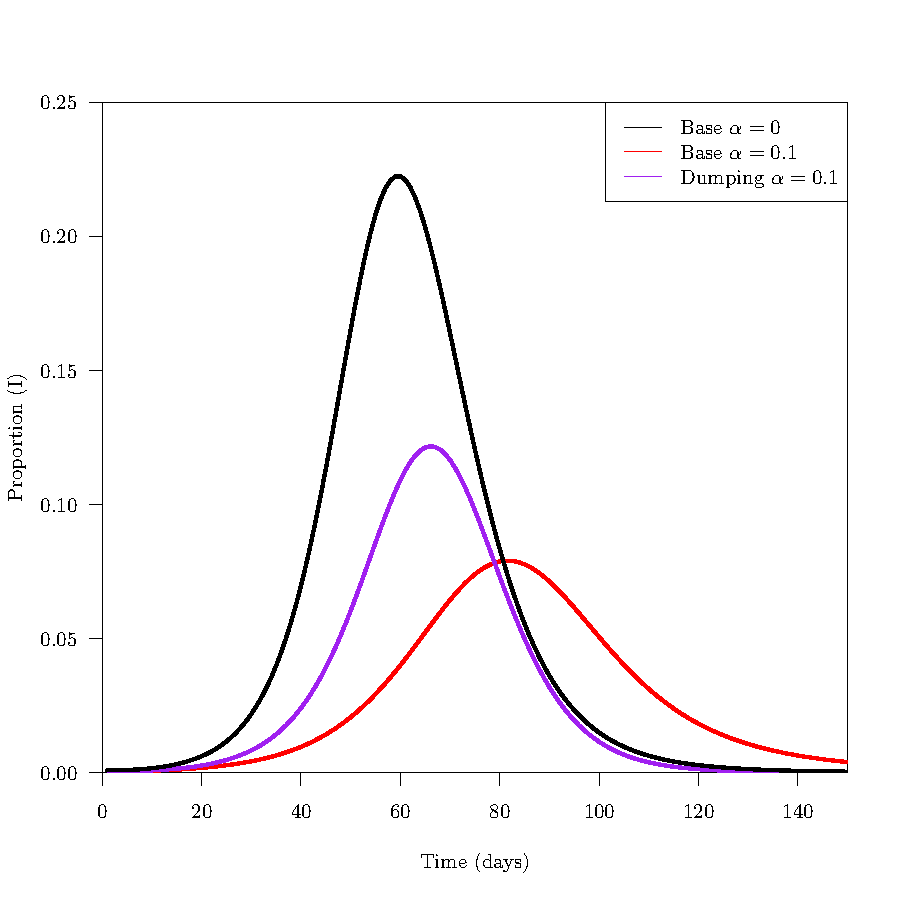
\includegraphics[width=0.95\textwidth]{images/centurytreatment.pdf}
\column{0.5\textwidth}
\begin{itemize}
\setlength\itemsep{2em}
\item Estimated death rate from cholera in the 19th century estimated to be up to $50\%$
\item Including disease induced death is ``beneficial" if death rate by cholera is high (Why?)
\item Improper sanitation increases peak prevalence
\end{itemize}
\end{columns}
\end{frame}


\begin{frame}{Treatment Strategies For Cholera}
\begin{enumerate}
\setlength\itemsep{2em}
\item Sanitation of Water
\item Vaccinations
\item Antibiotics
\end{enumerate}
\end{frame}

\begin{frame}{Sanitation of Water}
\begin{center}
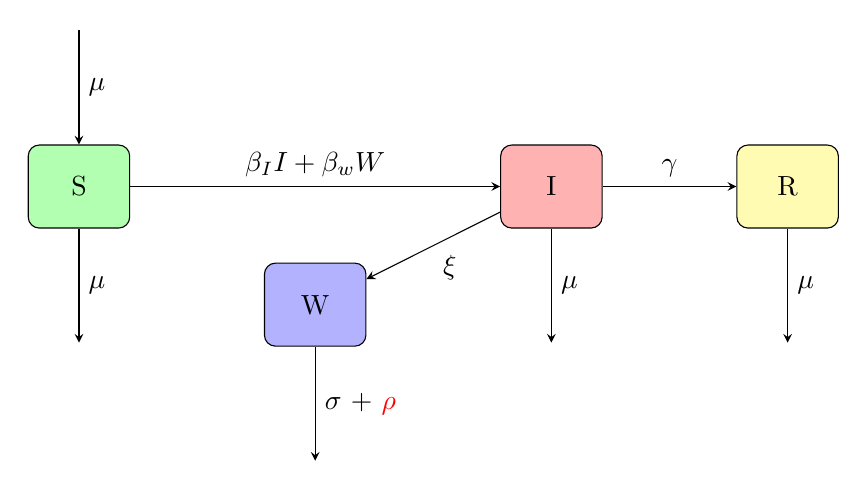
\begin{tikzpicture}[node distance=3cm, auto]

\node [blocks] (S) {S};
\node [blank, above of=S, yshift=-1cm] (0) { };
\node [blank, right of=S] (1) { };
\node [blockb, below of=1, yshift=1.5cm] (W) {W};
\node [blank, below of=W, yshift=1cm] (2) { };
\node [blocki, right of=1] (I) {I};
\node [blockr, right of=I] (R) {R};

\node [blank, below of=S, yshift=1cm] (3) {};
\node [blank, below of=I, yshift=1cm] (4) {};
\node [blank, below of=R, yshift=1cm] (5) {};

\path [line] (S) -- node {$\beta_I I + \beta_w W$} (I);
\path [line] (I) -- node {$\gamma$} (R);
\path [line] (I) -- node {$\xi$} (W);
\path [line] (W) -- node[anchor=west] {$\sigma$ + \textcolor{red}{$\rho$}} (2);
\path [line] (0) -- node[anchor=west] {$\mu$} (S);

\path [line] (S) -- node[anchor=west] {$\mu$} (3);
\path [line] (I) -- node[anchor=west] {$\mu$} (4);
\path [line] (R) -- node[anchor=west] {$\mu$} (5);

\end{tikzpicture}
\end{center}
\end{frame}

\begin{frame}{Vaccinations}
\begin{center}
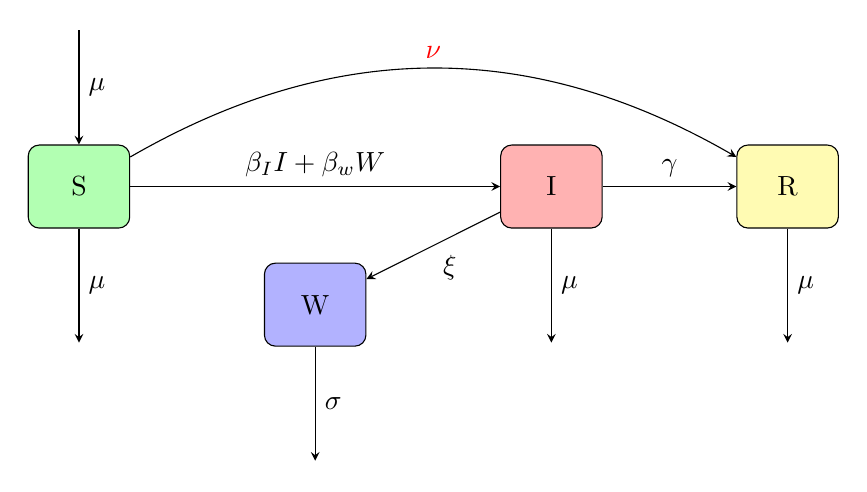
\begin{tikzpicture}[node distance=3cm, auto]

\node [blocks] (S) {S};
\node [blank, above of=S, yshift=-1cm] (0) { };
\node [blank, right of=S] (1) { };
\node [blockb, below of=1, yshift=1.5cm] (W) {W};
\node [blank, below of=W, yshift=1cm] (2) { };
\node [blocki, right of=1] (I) {I};
\node [blockr, right of=I] (R) {R};

\node [blank, below of=S, yshift=1cm] (3) {};
\node [blank, below of=I, yshift=1cm] (4) {};
\node [blank, below of=R, yshift=1cm] (5) {};

\path [line] (S) -- node {$\beta_I I + \beta_w W$} (I);
\path [line] (S) to [bend left,looseness=1] node[above] {\textcolor{red}{$\nu$}} (R);
\path [line] (I) -- node {$\gamma$} (R);
\path [line] (I) -- node {$\xi$} (W);
\path [line] (W) -- node[anchor=west] {$\sigma$} (2);
\path [line] (0) -- node[anchor=west] {$\mu$} (S);

\path [line] (S) -- node[anchor=west] {$\mu$} (3);
\path [line] (I) -- node[anchor=west] {$\mu$} (4);
\path [line] (R) -- node[anchor=west] {$\mu$} (5);

\end{tikzpicture}
\end{center}
\end{frame}

\begin{frame}{Antibiotics}
\begin{center}
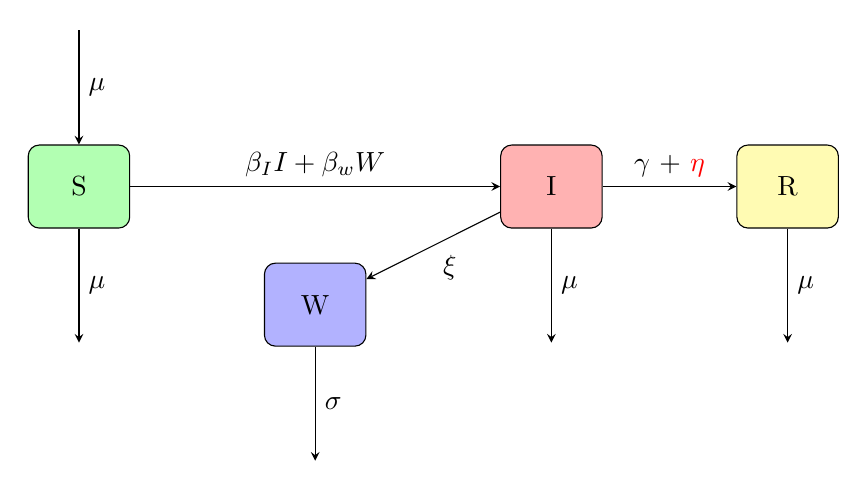
\begin{tikzpicture}[node distance=3cm, auto]

\node [blocks] (S) {S};
\node [blank, above of=S, yshift=-1cm] (0) { };
\node [blank, right of=S] (1) { };
\node [blockb, below of=1, yshift=1.5cm] (W) {W};
\node [blank, below of=W, yshift=1cm] (2) { };
\node [blocki, right of=1] (I) {I};
\node [blockr, right of=I] (R) {R};

\node [blank, below of=S, yshift=1cm] (3) {};
\node [blank, below of=I, yshift=1cm] (4) {};
\node [blank, below of=R, yshift=1cm] (5) {};

\path [line] (S) -- node {$\beta_I I + \beta_w W$} (I);
\path [line] (I) -- node {$\gamma$ + \textcolor{red}{$\eta$}} (R);
\path [line] (I) -- node {$\xi$} (W);
\path [line] (W) -- node[anchor=west] {$\sigma$} (2);
\path [line] (0) -- node[anchor=west] {$\mu$} (S);

\path [line] (S) -- node[anchor=west] {$\mu$} (3);
\path [line] (I) -- node[anchor=west] {$\mu$} (4);
\path [line] (R) -- node[anchor=west] {$\mu$} (5);

\end{tikzpicture}
\end{center}
\end{frame}

\begin{frame}{Comparing the Treatment Strategies}
\begin{columns}[onlytextwidth]
\column{0.5\textwidth}
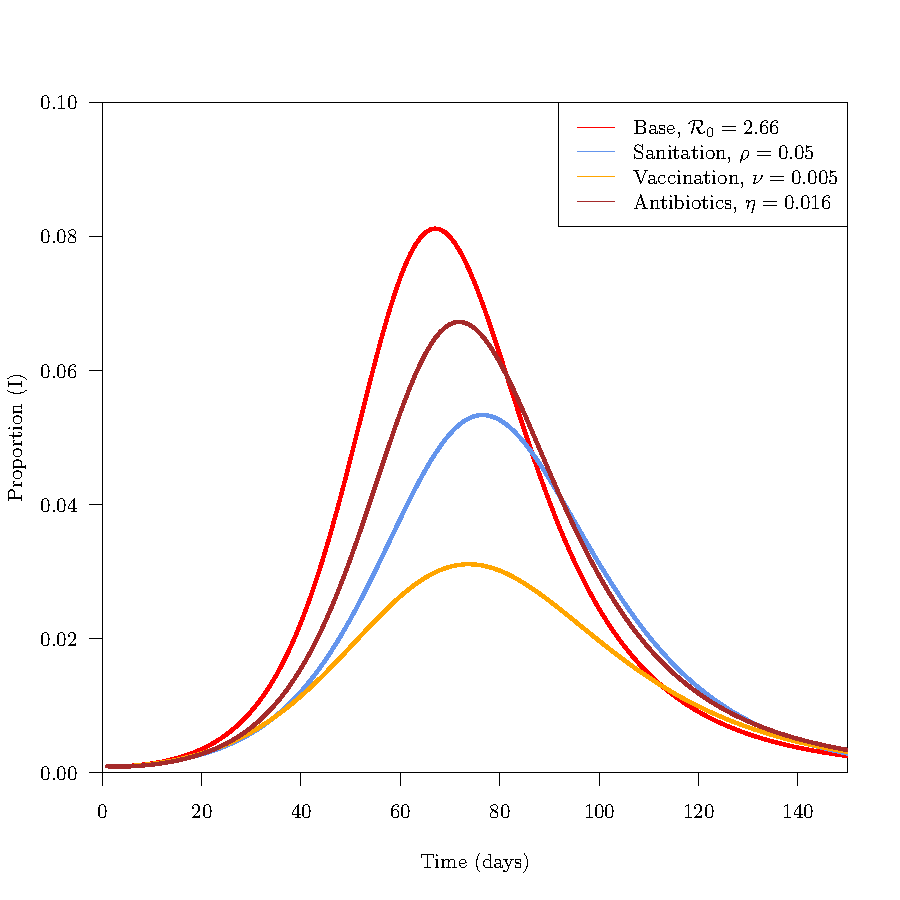
\includegraphics[width=0.95\textwidth]{images/treatcomparison.pdf}
\column{0.5\textwidth}
\begin{itemize}
\setlength\itemsep{2em}
\item Parameters chosen from literature
\item Lowest peak prevalence for vaccination treatment
\end{itemize}
\end{columns}
\end{frame}

\begin{frame}[t]{Multi-Patch Model}
\begin{align*}
    \frac{dS_i}{dt}&= \mu N - \mu S_i - \beta_i S_i I_i  - \beta_w S_i W_i + r(S)\\[1em]
    \frac{dI_i}{dt}&= \beta_i S_i I_i +  \beta_w S_i W_i - I_i (\gamma + \mu + \alpha) \\[1em]
    \frac{dR_i}{dt}&= \gamma I_i - \mu R_i + r(R)\\[1em]
    \frac{dW_i}{dt}&= \xi I_i - \sigma W_i + r(W)
\end{align*}
\end{frame}

\begin{frame}{Multi-Patch Model Assumptions}
\begin{itemize}
\setlength\itemsep{2em}
\item No dispersal of infected individuals
\item All patches have the same set of parameter values
\end{itemize}
\end{frame}


\begin{frame}{Spatial Dynamics (Base)}
    \begin{center}
    \pdfpcmovie{Base}{../sections/gifs/base.gif}
    \pdfpcmovie{Sanitation}{../sections/gifs/sanitation.gif}
    \pdfpcmovie{Antibiotics}{../sections/gifs/antibiotics.gif}
    \pdfpcmovie{Vaccination}{../sections/gifs/vaccination.gif}
\end{center}
\end{frame}

\begin{frame}{Comparing the Treatment Strategies In Multipatch Model}
    \begin{center}
    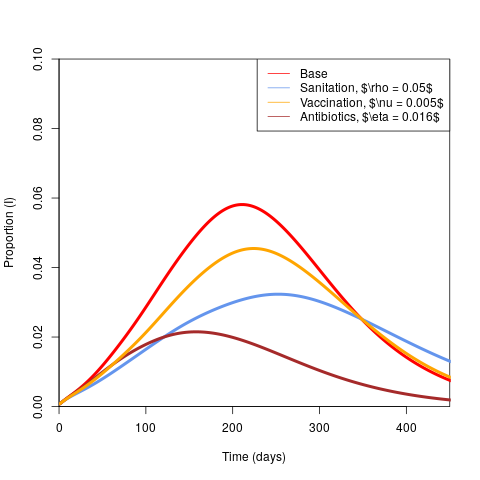
\includegraphics[width=0.7\textwidth]{images/spatialTreatments.png}
    \end{center}
\end{frame}



\begin{frame}{Conclusions and Further Research}
\begin{itemize}
\setlength\itemsep{2em}
\item 19th century outbreaks poorly handeled without antibiotics/vaccines
\item Different Treatments have different costs and outcomes
\item Further research on improving water sanitation effectivness to reduce reliance on vaccines/antibiotics
\end{itemize}
\end{frame}


\begin{frame}
\begin{center}
{\huge Thank you!}
\end{center}
\end{frame}


\begin{frame}[t,allowframebreaks]
  \frametitle{References}
    \nocite{*}
  \printbibliography
 \end{frame}

\end{document}
